\documentclass{article}
\usepackage{pgfplots}
\pgfplotsset{compat=1.17}

\begin{document}

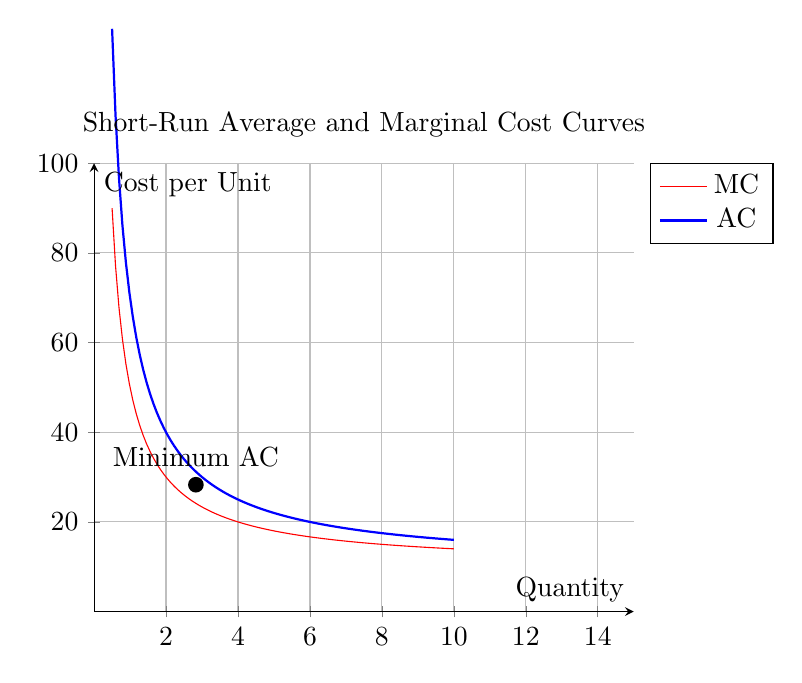
\begin{tikzpicture}
\begin{axis}[
    title={Short-Run Average and Marginal Cost Curves},
    xlabel={Quantity},
    ylabel={Cost per Unit},
    xmin=0, xmax=15,
    ymin=0, ymax=100,
    axis lines=middle,
    clip=false,
    grid=major,
    legend pos=outer north east,
]

% Marginal Cost Curve
\addplot[domain=0.5:10, samples=100, color=red] 
{10 + 40/x};
\addlegendentry{MC}

% Average Cost Curve
\addplot[domain=0.5:10, samples=100, color=blue, thick]
{(10 + 40/x) + 20*x/(x^2)};
\addlegendentry{AC}

% Highlight the minimum point of AC
\node[label={90:{Minimum AC}},circle,fill,inner sep=2pt] at (axis cs:2.83,28.3) {};

\end{axis}
\end{tikzpicture}

\end{document}
